
\documentclass[11pt]{article}
\date{}


    
    
    
    \usepackage[T1]{fontenc}
    % Nicer default font than Computer Modern for most use cases
    \usepackage{palatino}

    % Basic figure setup, for now with no caption control since it's done
    % automatically by Pandoc (which extracts ![](path) syntax from Markdown).
    \usepackage{graphicx}
    % We will generate all images so they have a width \maxwidth. This means
    % that they will get their normal width if they fit onto the page, but
    % are scaled down if they would overflow the margins.
    \makeatletter
    \def\maxwidth{\ifdim\Gin@nat@width>\linewidth\linewidth
    \else\Gin@nat@width\fi}
    \makeatother
    \let\Oldincludegraphics\includegraphics
    % Set max figure width to be 80% of text width, for now hardcoded.
    \renewcommand{\includegraphics}[1]{\Oldincludegraphics[width=.8\maxwidth]{#1}}
    % Ensure that by default, figures have no caption (until we provide a
    % proper Figure object with a Caption API and a way to capture that
    % in the conversion process - todo).
    \usepackage{caption}
    \DeclareCaptionLabelFormat{nolabel}{}
    \captionsetup{labelformat=nolabel}

    \usepackage{adjustbox} % Used to constrain images to a maximum size 
    \usepackage{xcolor} % Allow colors to be defined
    \usepackage{enumerate} % Needed for markdown enumerations to work
    \usepackage{geometry} % Used to adjust the document margins
    \usepackage{amsmath} % Equations
    \usepackage{amssymb} % Equations
    \usepackage{textcomp} % defines textquotesingle
    % Hack from http://tex.stackexchange.com/a/47451/13684:
    \AtBeginDocument{%
        \def\PYZsq{\textquotesingle}% Upright quotes in Pygmentized code
    }
    \usepackage{upquote} % Upright quotes for verbatim code
    \usepackage{eurosym} % defines \euro
    \usepackage[mathletters]{ucs} % Extended unicode (utf-8) support
    \usepackage[utf8x]{inputenc} % Allow utf-8 characters in the tex document
    \usepackage{fancyvrb} % verbatim replacement that allows latex
    \usepackage{grffile} % extends the file name processing of package graphics 
                         % to support a larger range 
    % The hyperref package gives us a pdf with properly built
    % internal navigation ('pdf bookmarks' for the table of contents,
    % internal cross-reference links, web links for URLs, etc.)
    \usepackage{hyperref}
    \usepackage{longtable} % longtable support required by pandoc >1.10
    \usepackage{booktabs}  % table support for pandoc > 1.12.2
    \usepackage[normalem]{ulem} % ulem is needed to support strikethroughs (\sout)
                                % normalem makes italics be italics, not underlines
    

    
    % Colors for the hyperref package
    \definecolor{urlcolor}{rgb}{0,.145,.698}
    \definecolor{linkcolor}{rgb}{.71,0.21,0.01}
    \definecolor{citecolor}{rgb}{.12,.54,.11}

    % ANSI colors
    \definecolor{ansi-black}{HTML}{3E424D}
    \definecolor{ansi-black-intense}{HTML}{282C36}
    \definecolor{ansi-red}{HTML}{E75C58}
    \definecolor{ansi-red-intense}{HTML}{B22B31}
    \definecolor{ansi-green}{HTML}{00A250}
    \definecolor{ansi-green-intense}{HTML}{007427}
    \definecolor{ansi-yellow}{HTML}{DDB62B}
    \definecolor{ansi-yellow-intense}{HTML}{B27D12}
    \definecolor{ansi-blue}{HTML}{208FFB}
    \definecolor{ansi-blue-intense}{HTML}{0065CA}
    \definecolor{ansi-magenta}{HTML}{D160C4}
    \definecolor{ansi-magenta-intense}{HTML}{A03196}
    \definecolor{ansi-cyan}{HTML}{60C6C8}
    \definecolor{ansi-cyan-intense}{HTML}{258F8F}
    \definecolor{ansi-white}{HTML}{C5C1B4}
    \definecolor{ansi-white-intense}{HTML}{A1A6B2}

    % commands and environments needed by pandoc snippets
    % extracted from the output of `pandoc -s`
    \providecommand{\tightlist}{%
      \setlength{\itemsep}{0pt}\setlength{\parskip}{0pt}}
    \DefineVerbatimEnvironment{Highlighting}{Verbatim}{commandchars=\\\{\}}
    % Add ',fontsize=\small' for more characters per line
    \newenvironment{Shaded}{}{}
    \newcommand{\KeywordTok}[1]{\textcolor[rgb]{0.00,0.44,0.13}{\textbf{{#1}}}}
    \newcommand{\DataTypeTok}[1]{\textcolor[rgb]{0.56,0.13,0.00}{{#1}}}
    \newcommand{\DecValTok}[1]{\textcolor[rgb]{0.25,0.63,0.44}{{#1}}}
    \newcommand{\BaseNTok}[1]{\textcolor[rgb]{0.25,0.63,0.44}{{#1}}}
    \newcommand{\FloatTok}[1]{\textcolor[rgb]{0.25,0.63,0.44}{{#1}}}
    \newcommand{\CharTok}[1]{\textcolor[rgb]{0.25,0.44,0.63}{{#1}}}
    \newcommand{\StringTok}[1]{\textcolor[rgb]{0.25,0.44,0.63}{{#1}}}
    \newcommand{\CommentTok}[1]{\textcolor[rgb]{0.38,0.63,0.69}{\textit{{#1}}}}
    \newcommand{\OtherTok}[1]{\textcolor[rgb]{0.00,0.44,0.13}{{#1}}}
    \newcommand{\AlertTok}[1]{\textcolor[rgb]{1.00,0.00,0.00}{\textbf{{#1}}}}
    \newcommand{\FunctionTok}[1]{\textcolor[rgb]{0.02,0.16,0.49}{{#1}}}
    \newcommand{\RegionMarkerTok}[1]{{#1}}
    \newcommand{\ErrorTok}[1]{\textcolor[rgb]{1.00,0.00,0.00}{\textbf{{#1}}}}
    \newcommand{\NormalTok}[1]{{#1}}
    
    % Additional commands for more recent versions of Pandoc
    \newcommand{\ConstantTok}[1]{\textcolor[rgb]{0.53,0.00,0.00}{{#1}}}
    \newcommand{\SpecialCharTok}[1]{\textcolor[rgb]{0.25,0.44,0.63}{{#1}}}
    \newcommand{\VerbatimStringTok}[1]{\textcolor[rgb]{0.25,0.44,0.63}{{#1}}}
    \newcommand{\SpecialStringTok}[1]{\textcolor[rgb]{0.73,0.40,0.53}{{#1}}}
    \newcommand{\ImportTok}[1]{{#1}}
    \newcommand{\DocumentationTok}[1]{\textcolor[rgb]{0.73,0.13,0.13}{\textit{{#1}}}}
    \newcommand{\AnnotationTok}[1]{\textcolor[rgb]{0.38,0.63,0.69}{\textbf{\textit{{#1}}}}}
    \newcommand{\CommentVarTok}[1]{\textcolor[rgb]{0.38,0.63,0.69}{\textbf{\textit{{#1}}}}}
    \newcommand{\VariableTok}[1]{\textcolor[rgb]{0.10,0.09,0.49}{{#1}}}
    \newcommand{\ControlFlowTok}[1]{\textcolor[rgb]{0.00,0.44,0.13}{\textbf{{#1}}}}
    \newcommand{\OperatorTok}[1]{\textcolor[rgb]{0.40,0.40,0.40}{{#1}}}
    \newcommand{\BuiltInTok}[1]{{#1}}
    \newcommand{\ExtensionTok}[1]{{#1}}
    \newcommand{\PreprocessorTok}[1]{\textcolor[rgb]{0.74,0.48,0.00}{{#1}}}
    \newcommand{\AttributeTok}[1]{\textcolor[rgb]{0.49,0.56,0.16}{{#1}}}
    \newcommand{\InformationTok}[1]{\textcolor[rgb]{0.38,0.63,0.69}{\textbf{\textit{{#1}}}}}
    \newcommand{\WarningTok}[1]{\textcolor[rgb]{0.38,0.63,0.69}{\textbf{\textit{{#1}}}}}
    
    
    % Define a nice break command that doesn't care if a line doesn't already
    % exist.
    \def\br{\hspace*{\fill} \\* }
    % Math Jax compatability definitions
    \def\gt{>}
    \def\lt{<}
    % Document parameters
    
\title{Calibración de cámaras con OpenCV}

    
    
\author{Sergio Agudelo}

    

    
    % Prevent overflowing lines due to hard-to-break entities
    \sloppy 
    % Setup hyperref package
    \hypersetup{
      breaklinks=true,  % so long urls are correctly broken across lines
      colorlinks=true,
      urlcolor=urlcolor,
      linkcolor=linkcolor,
      citecolor=citecolor,
      }
    % Slightly bigger margins than the latex defaults
    
    \geometry{verbose,tmargin=1in,bmargin=1in,lmargin=1in,rmargin=1in}
    
    

    \begin{document}
    
    
    \maketitle
    
    

    
    \section{Introducción}\label{introducciuxf3n}

    Todo sistema en algún grado inteligente depende absolutamente de la
realimentación que recibe de su entorno. Es decir, el funcionamiento
correcto o incorrecto de los sensores que posea es crucial para su
eficaz funcionamiento. Luego, es preciso calibrar aquellos sensores para
conocer su comportamiento bajo distintas condiciones ambientales, y así
obrar adecuadamente a la hora de diseñar el sistema que realizamos.
Desafortunadamente, en el caso de los sensores ópticos (cámaras) ocurre
que es complejo determinar de forma directa las variables de interés en
la calibración (no son usualmente suministradas por el fabricante,
adicionalmente, medirlas experimentalmente no es una tarea fácil). Sin
embargo, usando modelos geométricos y matemáticos existentes, es posible
obtener los parámetros de calibración de una cámara de forma indirecta.
Este documento pretende ilustrar el modelo más sencillo que se concibe
de una cámara, y luego demostrar el proceso de calbración usando la
librería \href{http://opencv.org}{OpenCV} (cuyas funciones se basan en
el modelo mencionado).

    \subsection{\texorpdfstring{El modelo \emph{pinhole}
\cite{bradski2008learning}}{El modelo pinhole }}\label{el-modelo-pinhole}

    Este modelo de cámara consiste en un plano con una apertura puntual en
su centro, sobre la que sólo puede pasar un rayo de luz. De esta manera,
sólo un rayo que parta de algún punto específico del espacio puede
entrar. Paralelo a este plano, existe otro plano, que es el que
capturará los rayos proyectados, formándose así una imagen.

    \begin{figure}[htbp]
\centering
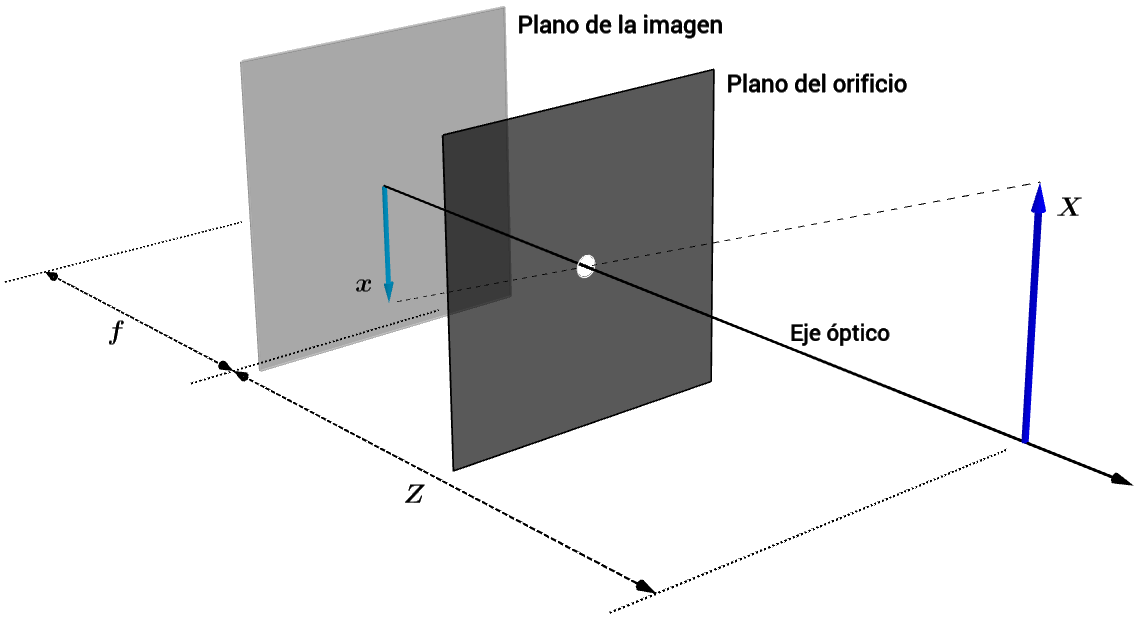
\includegraphics{img/1-fig1.png}
\caption{Modelo pinhole: los rayos proyectados a través de la apertura
forman una imagen.}
\end{figure}

    La distancia \(f\) es conocida como \emph{distancia focal} y \(Z\) es la
distancia entre cámara y objeto. Para simplificar los cálculos
necesarios en la solución de el sistema coordenado de la anterior
imagen, se reorganiza todo así:

    \begin{figure}[htbp]
\centering
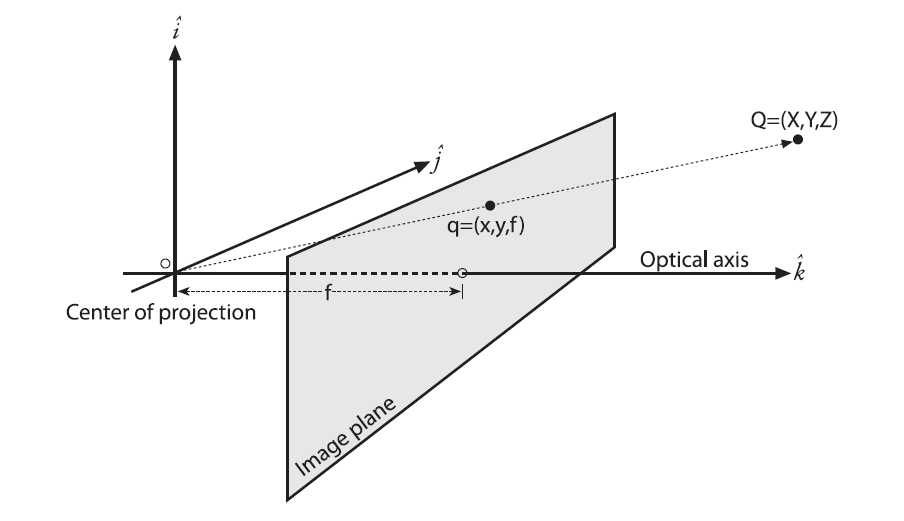
\includegraphics{img/1-fig2.png}
\caption{Modelo usado para la solución algebraica. Nótese la
diferenciación entre coordenadas \(x\),\(y\) (imagen) y
\(X\),\(Y\),\(Z\) (espacio)}
\end{figure}

    El mapeo \(f:\ Q \mapsto q\) corresponde a la siguiente función:

    \[f\left(X,Y,Z\right) = \left(f_x\left(\frac{X}{Z}\right)+c_x,\ f_y\left(\frac{Y}{Z}\right)+c_y\right)\]

    En donde,

\begin{equation} \label{eq:mapx}
    x_{imagen} = f_x\left(\frac{X}{Z}\right)+c_x
\end{equation}\begin{equation} \label{eq:mapy}
    y_{imagen} = f_y\left(\frac{Y}{Z}\right)+c_y
\end{equation}

    La figura ilustra lo que sería un modelo ideal, en que el plano de la
imagen es paralelo al plano \(\hat{i}\hat{j}\), y el eje \(\hat{k}\)
interseca al plano de la imagen en su centro. En la construcción de una
cámara, lograr una alineación perfecta es imposible. Por ello, se
introducen las variables \(c_x\) y \(c_y\), las cuales representan
desplazamientos respectivamente horizontal y vertical del eje óptico
respecto al centro del plano. También se introducen dos distancias
focales, \(f_x\) y \(f_y\), debido a que los sensores ópticos no poseen
pixeles cuadrados, en realidad son rectangulares.

    Reorganizando las ecuaciones \ref{eq:mapx} y \ref{eq:mapy},

    \[x_{imagen} Z = f_x X + c_x Z\] \[y_{imagen} Z = f_y Y + c_y Z\]

    Es conveniente expresar estas ecuaciones de forma matricial usando
coordenadas homogéneas, de la forma \(q = MQ\), en donde

    \begin{center}
$q =
\begin{bmatrix}
    x \\[0.3em]
    y \\[0.3em]
    w
\end{bmatrix}$ , 
$M = 
\begin{bmatrix}
f_x &  0  & c_x  \\[0.3em]
 0  & f_y & c_y  \\[0.3em]
 0  &  0  &  1
\end{bmatrix}$ ,
$Q =
\begin{bmatrix}
    X \\[0.3em]
    Y \\[0.3em]
    Z
\end{bmatrix}$
\end{center}

    \subsubsection{Distorsión de los
lentes}\label{distorsiuxf3n-de-los-lentes}

    Varios supuestos deben olvidarse, y reemplazarse por modelos, para poder
llegar a una representación más precisa y generalizada. No se consideró
previamente, pero los sensores ópticos de una cámara (CCDs, o
dispositivos de carga acoplada, son los más ampliamente usados) poseen
una alta integración en una área muy reducida,


    % Add a bibliography block to the postdoc
    
    
\bibliographystyle{plain}
\bibliography{refs}

    
    \end{document}
